\chapter{Konzeption}
\section{Szenarien}
Die Szenarien haben eine ungeregelte Kreuzung gemeinsam. Ziel ist es, dass das Fahrzeug eine Kreuzung erkennt sowie mit potenziellem Gegenverkehr umgehen kann. Das Fahrzeug soll 
erkennen, in welche Richtungen es abbiegen darf, sich für eine Richtung entscheiden und das entsprechende Fahrmannöver ausführen. Zusätzlich sollen die odometrischen Koordinaten
der Schlüsselpunkte einer Kreuzung berechnet werden. Das bedeutet, dass Start- sowie Endpunkte eines Fahrmannövers bekannt sein sollen. 
\paragraph{Szenario 1}
\label{Szenario 1}
Das Fahrzeug erkennt eine ungeregelte Kreuzung, bei der es keinen weiteren Verkehr gibt. Es ist ein grundsätzliches Szenario und soll als Test dienen, dass der Roboter die grundlegende
Fähigkeit verfügt, eine Kreuzung zu erkennen und das entsprechende Fahrmannöver durchzuführen.

\paragraph{Szenario 2}
\label{Szenario 2}
Das Fahrzeug erkennt eine ungeregelte Kreuzung sowie ein weiteres Fahrzeug, welches sich direkt vor ihm befindet. Das andere Fahrzeug soll erkannt und ein entsprechender Sicherheitsabstand 
eingehalten werden. Wenn die Kreuzung frei ist, soll das Fahrzeug entsprechend \ref{Szenario 1} fortfahren.

\paragraph{Szenario 3}
\label{Szenario 3}
Das Fahrzeug erkennt eine ungeregelte Kreuzung, sowie ein weiteres Fahrzeug, welches aus der rechten Fahrtrichtung kommt. Entsprechend der Straßenverkehrsordnung soll hier die 
Regel "rechts vor links" beachtet werden. Das Fahrzeug soll deshalb warten, bis das andere Fahrzeug die Kreuzung verlassen hat.

\paragraph{Szenario 4}
\label{Szenario 4}
Das Fahrzeug erkennt eine ungeregelte Kreuzung, sowie ein weiteres Fahrzeug, welches aus der linken Fahrtrichtung kommt. Entgegen \ref{Szenario 3} soll das 
Fahrzeug hier also sein Vorfahrtsrecht beachten.

\paragraph{Szenario 5}
\label{Szenario 5}
Das Fahrzeug erkennt eine ungeregelte Kreuzung, sowie ein weiteres liegengebliebendes Fahrzeug, welches die gewünschte Fahrtrichtung blockiert. Das Fahrzeug soll die Fahrt in eine andere
Richtung fortsetzen.

\section{Voraussetzungen}
Die Arbeit beruht wie bereits beschrieben auf dem AutoRace-Projekt. Somit ist die erste Voraussetzung, dass die Fahrbahnen unidirektional sind. Im Detail bedeutet dies, dass
der Roboter anhand der Fahrbahnbegrenzung erkennen kann, in welche Richtungen abgebogen werden darf. Für die Detektion von Gegenverkehr bedeutet dies, dass lediglich aus Richtungen,
in die nicht abgebogen werden darf, Gegenverkehr zu erwarten ist.

Zusätzlich wird angenommen, dass die Fahrbahnbegrenzung wie bereits beschrieben rechts weiß und links gelb ist. Darauf aufbauend wird definiert, dass eine Kreuzung nicht unmittelbar
nach einer Kurve beginnt. Der Roboter muss die Chance haben, die Kreuzung zu erkennen. Da die Kamera erhöht verbaut ist, hat der Roboter ein totes Sichtfeld und hätte somit keine Möglichkeit
eine Kreuzung visuell zu erkennen, wenn diese unmittelbar nach einer Kurve beginnt.
Eine Möglichkeit, die durch das AutoRace-Projekt besteht, ist eine Erkennung einer Kreuzung durch Schilder. Ähnlich zur realen Welt hätten hier Vorfahrsschilder 
oder neu entworfene Schilder genutzt werden können. Durch den beschriebenen Objekterkennungsansatz mit z.B. SIFT und FLANN besteht hier die Möglichkeit, eine Kreuzung direkt zu erkennen.
Dies würde dazu führen, dass ein Kreuzungsszenario sicher eingeleitet werden kann. Jedoch hat dieser Ansatz zwei wesentliche Nachteile. Zunächst fehlen dem Roboter sämtliche Informationen
über die Kreuzung, wie z.B. die Richtungen in die er abbiegen darf oder aber die Schlüsselpunkte. Ein weiterer Nachteil ist, dass es zusätzlichen Aufwand bei einer potenziellen
Nutzung in der Realität bedeutet. Wenn an jeder Kreuzung Schilder stehen müssen, büßt die Software an Flexibilität ein.
Aus diesen Gründen gilt die Voraussetzung, dass eine Krezung ausschließlich durch die Fahrbahnmakierung identifiziert wird.

Zur Kommunikation zwischen den Robotern wird die Abwandlung von Connected Cars als gegeben angesehen. Jeder Roboter, der in den Szenarien eingesetzt wird, kann mit allen anderen
Robotern kommunizieren. Das bedeutet, dass z.B. auch ein liegengebliebender Roboter stehts seine Daten übermittelt und hierüber identifiziert werden kann.

\section{Versuchsaufbau}
Um die einzelnen Szenarien in Gazebo zu simulieren, wurden neue Simulationswelten bereitgestellt. Grundsätzlich basieren diese Welten auf der Simulation des TurlteBot AutoRace 2017.
Der wesentliche Unterschied ist, dass sämtliche Aufgaben entfallen. Das bedeutet, dass die Ampel, der Parkplatz, der Tunnel sowie die Zollschranke entfernt wurden. Grundsätzlich
ist die Version des AutoRace, auf der der Versuchsaufbau basiert, nicht relevant, da für die Arbeit lediglich die Fahrbahn benötigt wird. Diese hat sich in den letzten Jahren nicht
verändert.

Insgesamt wurden drei neue Welten entworfen. Die erste ist in Abbildung \ref{fig:Testworld_Map} zu sehen. Hier sind verschiedene Kreuzungen dargestellt. Die Intention ist hier,
dass der Roboter am roten Pfeil in der entsprechenden Richtung startet. Bei jeder Kreuzung soll er erkennen, welche Richtungen für ein Abbiegemannöver erlaubt sind. Wenn die Detektion
erfolgreich funktioniert, soll der Roboter das entsprechende Mannöver für jede erlaubte Richtung in separaten Durchlaufen durchführen. Eine Alternative, um die Detektion zu prüfen, wäre
den Roboter auf statischen Kameraaufnahmen arbeiten zu lassen. Diese Kameraaufnahmen hätten mit entsprechenden Informationen beschrieben werden müssen, welche Richtungen erlaubt sind oder
an welchen Koordinaten sich die Schlüsselpunkte der Kreuzung befinden. Zweiteres ist direkt abhängig von der aktuellen Position des Roboters, was die Arbeit mit statischen Bildern
erschwert. Ein zusätzliches Manko ist, dass sich das statische Bild nicht verändert. Wie später zu sehen sein wird, zeigt die Realität, dass sich selbst beim Stillstand des Roboters in der
simulierten Welt das aufgenommene Bild minimal verändert. Dieses Verhalten ist auch für die reale Welt anzunehmen, da beispielsweise die Vibration durch verbaute Geräte am TurtleBot 3
ausreichen würde, um Varianzen in einer Bildsequenz zu haben.

In dieser Simulation sind noch keine anderen Roboter enthalten. In dieser Welt soll ausschließlich die Kernfunktionalität, die Detektion und das Durchführen der Abbiegemannöver, 
simuliert und erprobt werden. Die Implementierung ist an dieser Stelle noch unabhängig vom AutoRace-Projekt, weshalb dieser Versuch auf neuentwickelten Nodes beruht. 

\begin{figure}[h!]
  \centering
  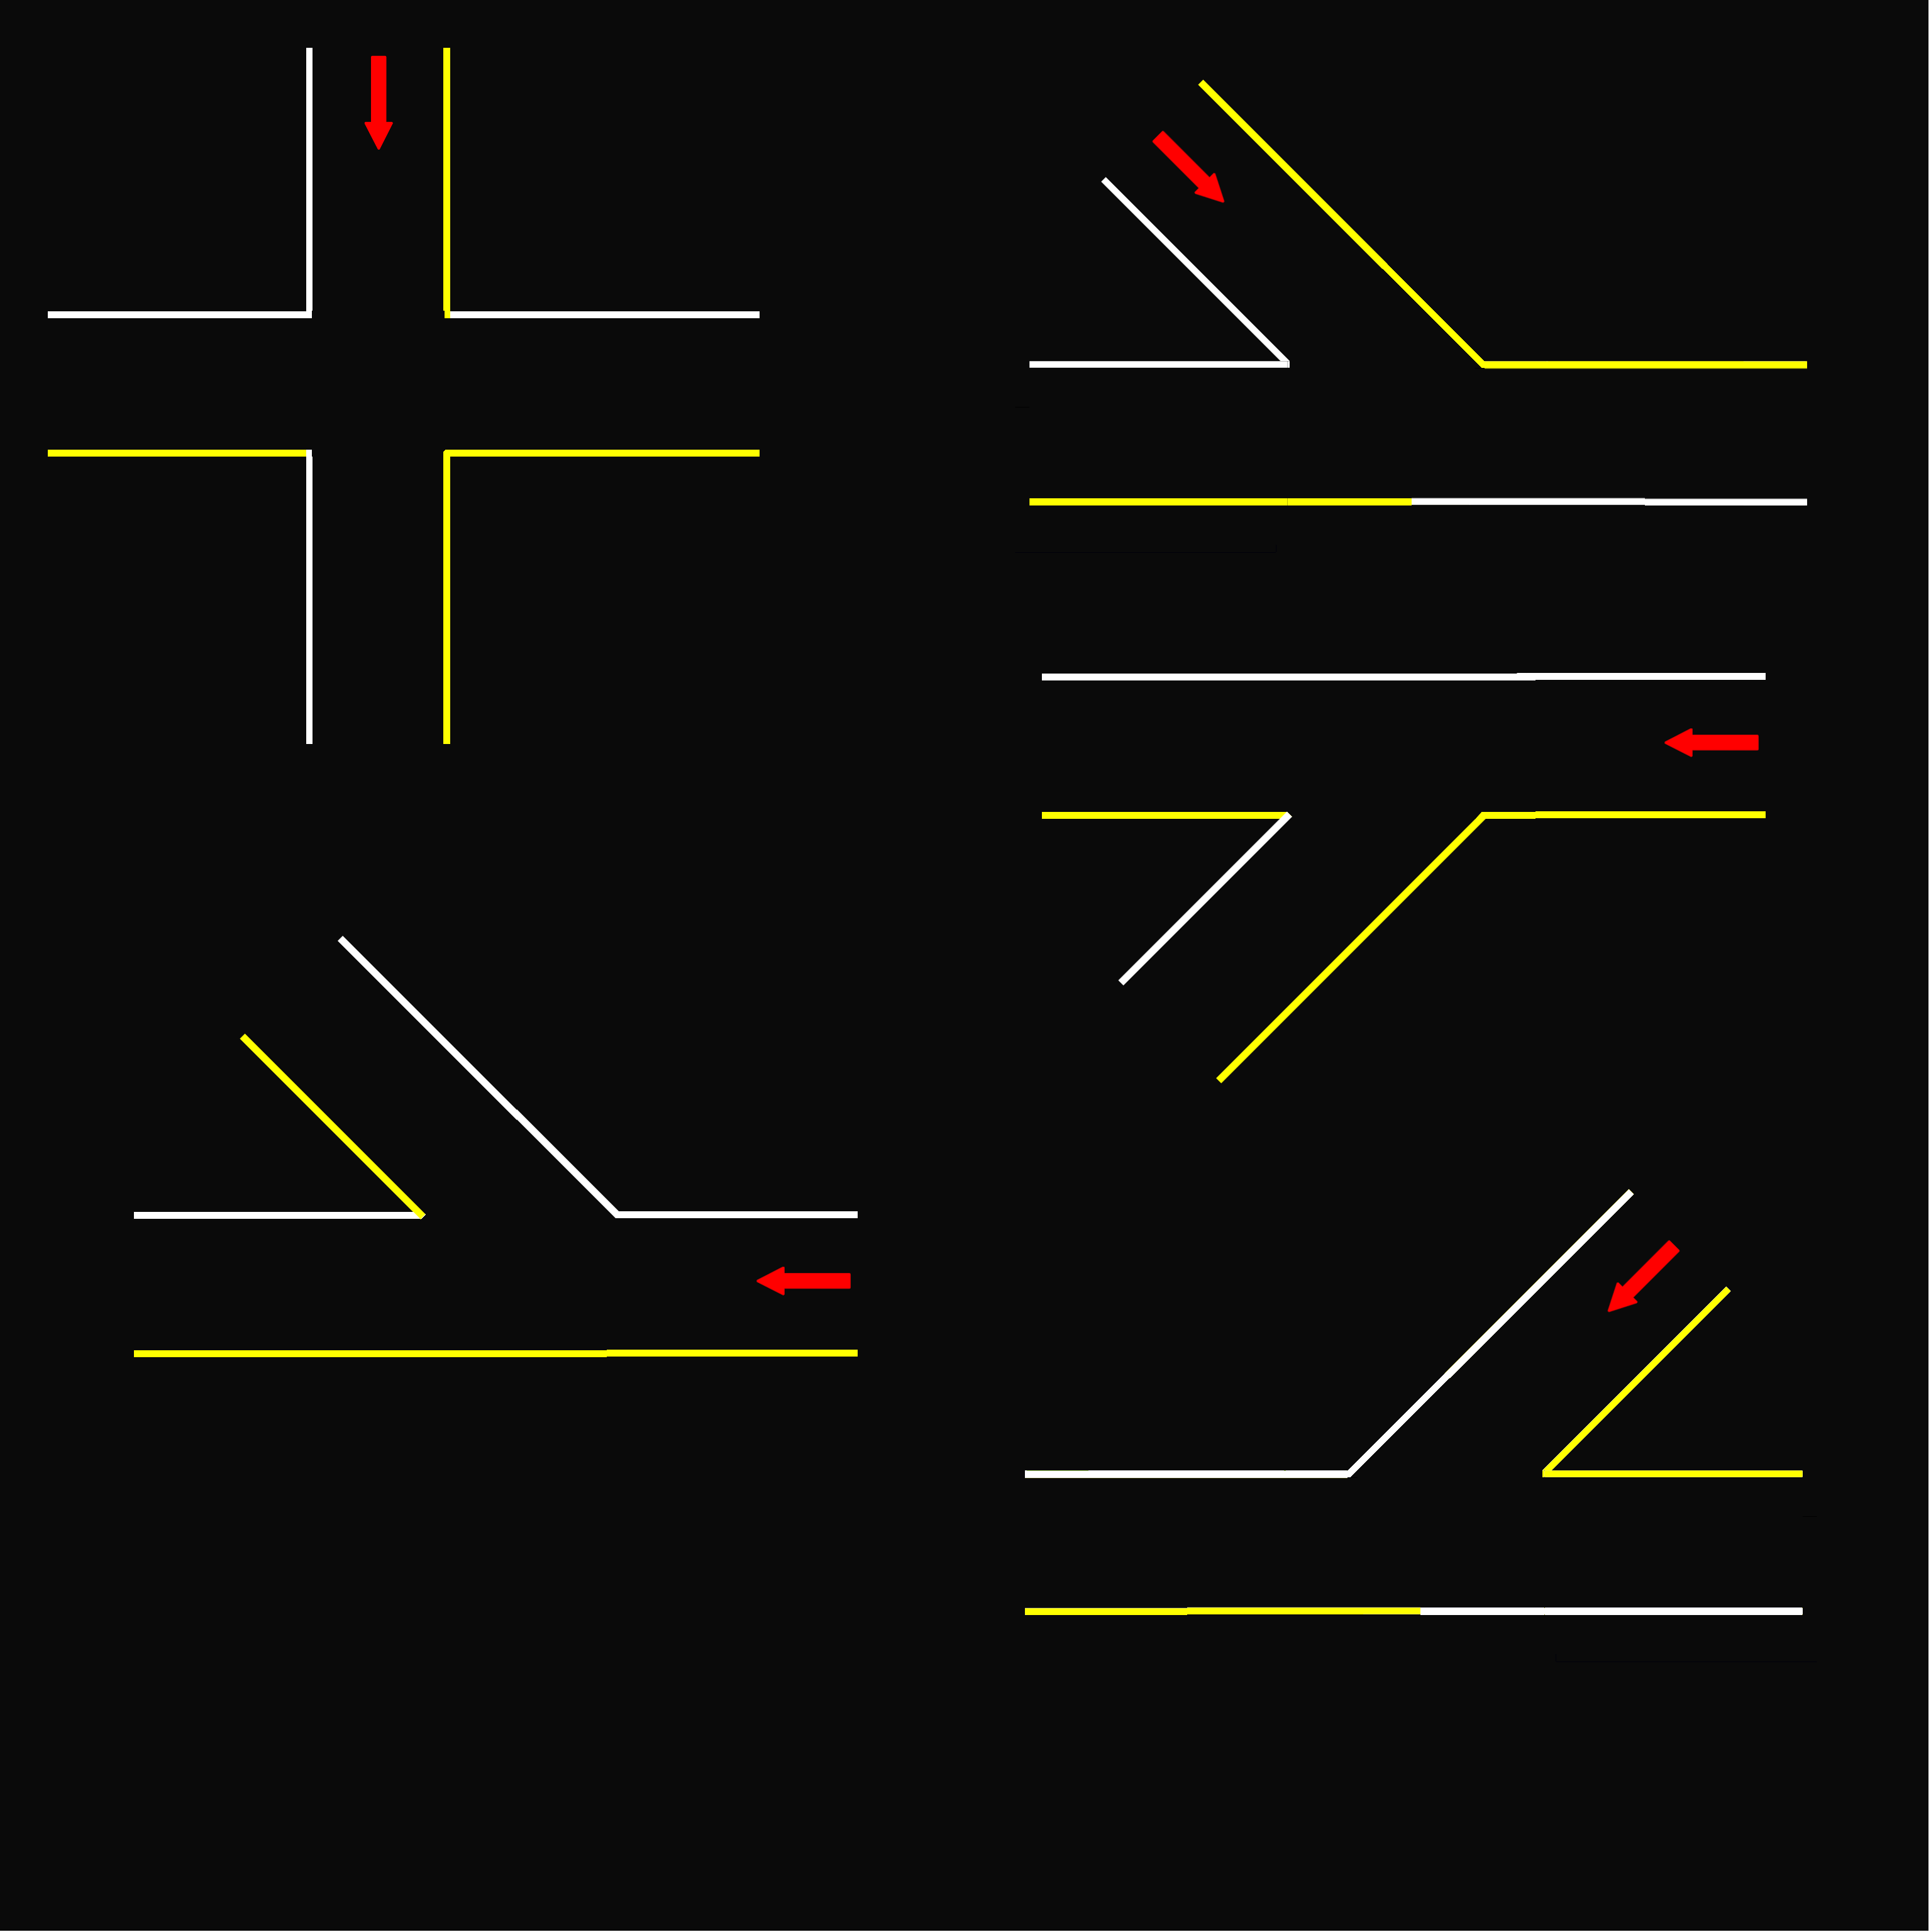
\includegraphics[height=0.5\textwidth]{images/road_test_map.png}
  \caption{Karte der Testwelt}
  \label{fig:Testworld_Map}
\end{figure}

Die zweite Welt ist in Abbildung \ref{fig:Testworld_Autorace_Map} zu sehen. Hier sollen die einzelnen Szenarien getrennt simuliert und erprobt werden. Der erste Versuch wird darin bestehen,
die neuentwickelten Nodes sowie die bestehende AutoRace-Implementierung zusammenzuführen. Der Roboter soll also die Spur halten, bis er eine Kreuzung erkennt und entsprechend den Modus
wechseln. In diesem Modus soll er entsprechende Fahrmannöver an der Kreuzung durchführen. Nachdem dies absolviert ist, soll der Roboter wieder in den entsprechenden Modus wechseln,
um die Fahrspur zu halten.

Im nächsten Schritt sollen in dieser Welt mehrere Instanzen des TurtleBot 3 fahren. Hier soll das Verhalten entsprechend der Szenarien von den Robotern durchgeführt werden. Hier ist das Ziel,
dass das Verhalten an einem rudimentären Beispiel getestet werden kann.

Der Hauptfokus in dieser Welt soll darauf liegen, dass die Robustheit des Roboters getestet werden kann. Wenn die Implementierung bereit ist, soll der Roboter für längere Zeit in der
Welt fahren. Wenn die Software robust ist, dann wird der Roboter für die ganze Durchführungsdauer die Spur halten können und sich an den Kreuzungen richtig verhalten.

\begin{figure}[h!]
    \centering
    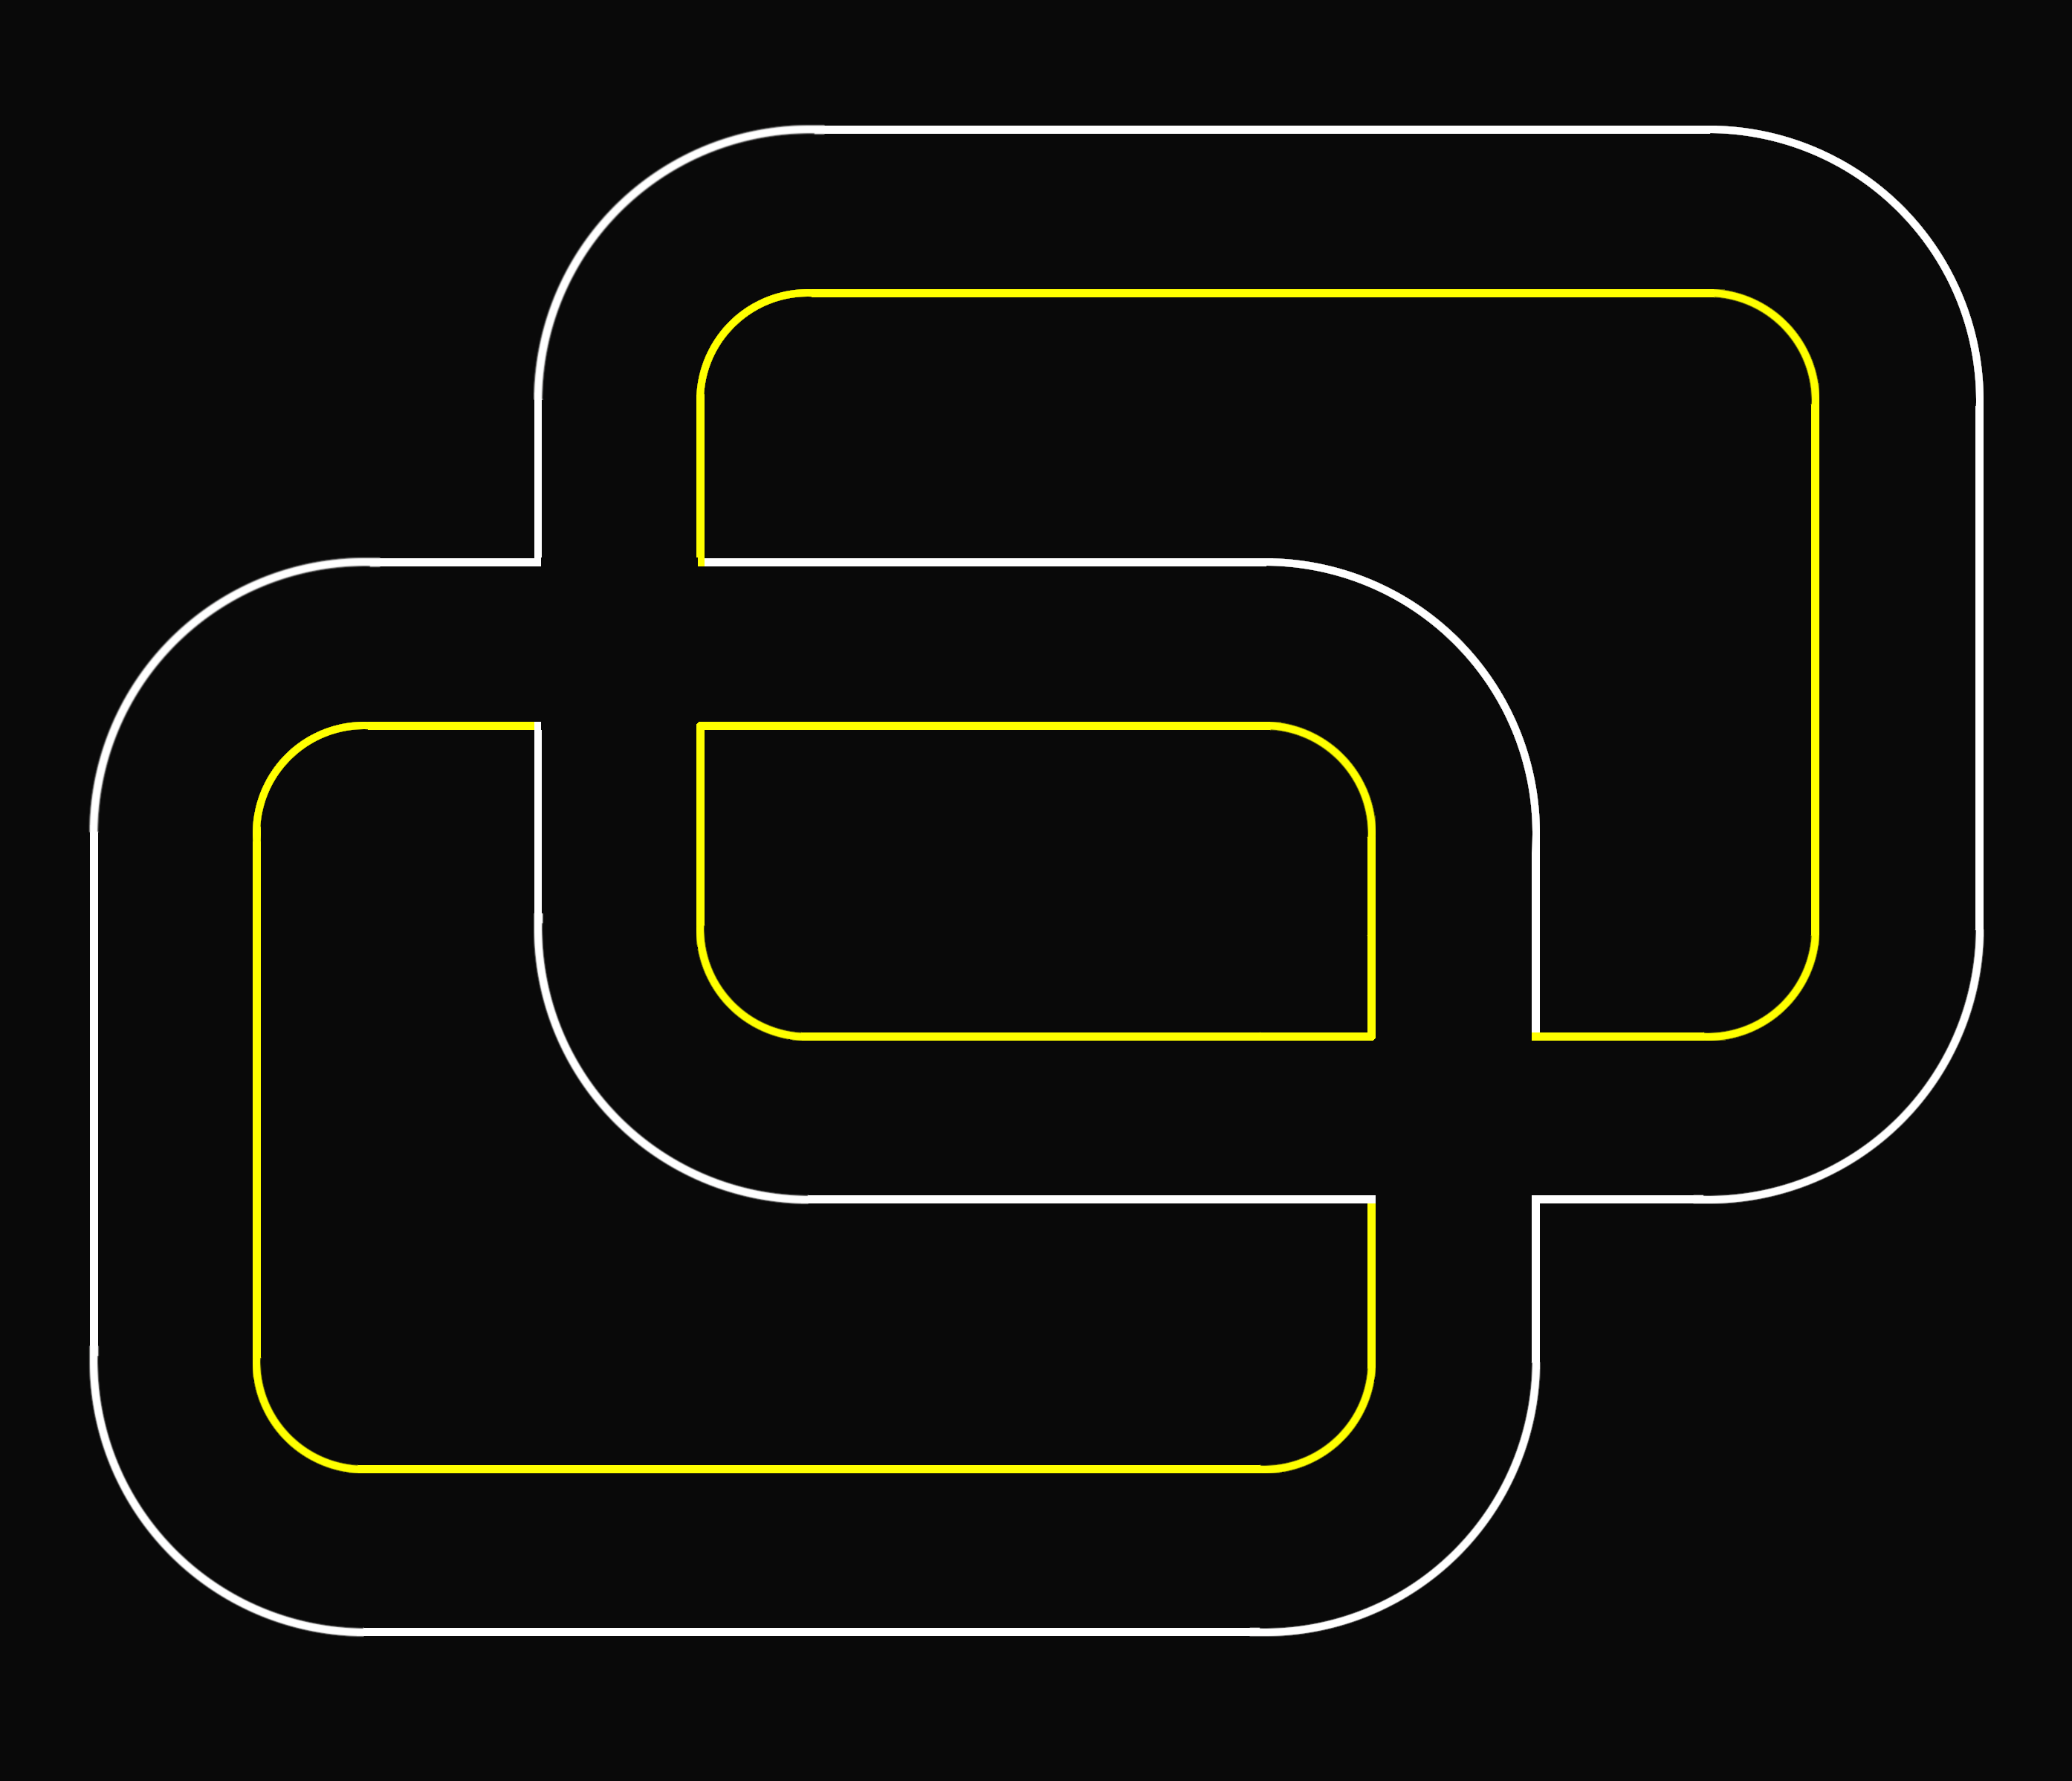
\includegraphics[height=0.5\textwidth]{images/road_autorace_map.png}
    \caption{Karte der Testwelt mit Straßennetz}
    \label{fig:Testworld_Autorace_Map}
  \end{figure}

  Die letzte Welt ist in Abbildung \ref{fig:Testworld_Final_Map} zu sehen. In dieser Welt sind komplexere Kreuzungsszenarien mit aufgenommen. Auch hier ist das Ziel, die Robustheit der Software zu prüfen, 
  indem mehrere Instanzen des TurtleBot 3 versuchen, durch das Straßennetz zu navigieren ohne von der Spur abzukommen oder mit einem anderen TurtleBot zu kollidieren.

  Die einzelnen Szenarien werden auch hier manuell nachgestellt und erprobt.

\begin{figure}[h!]
  \centering
  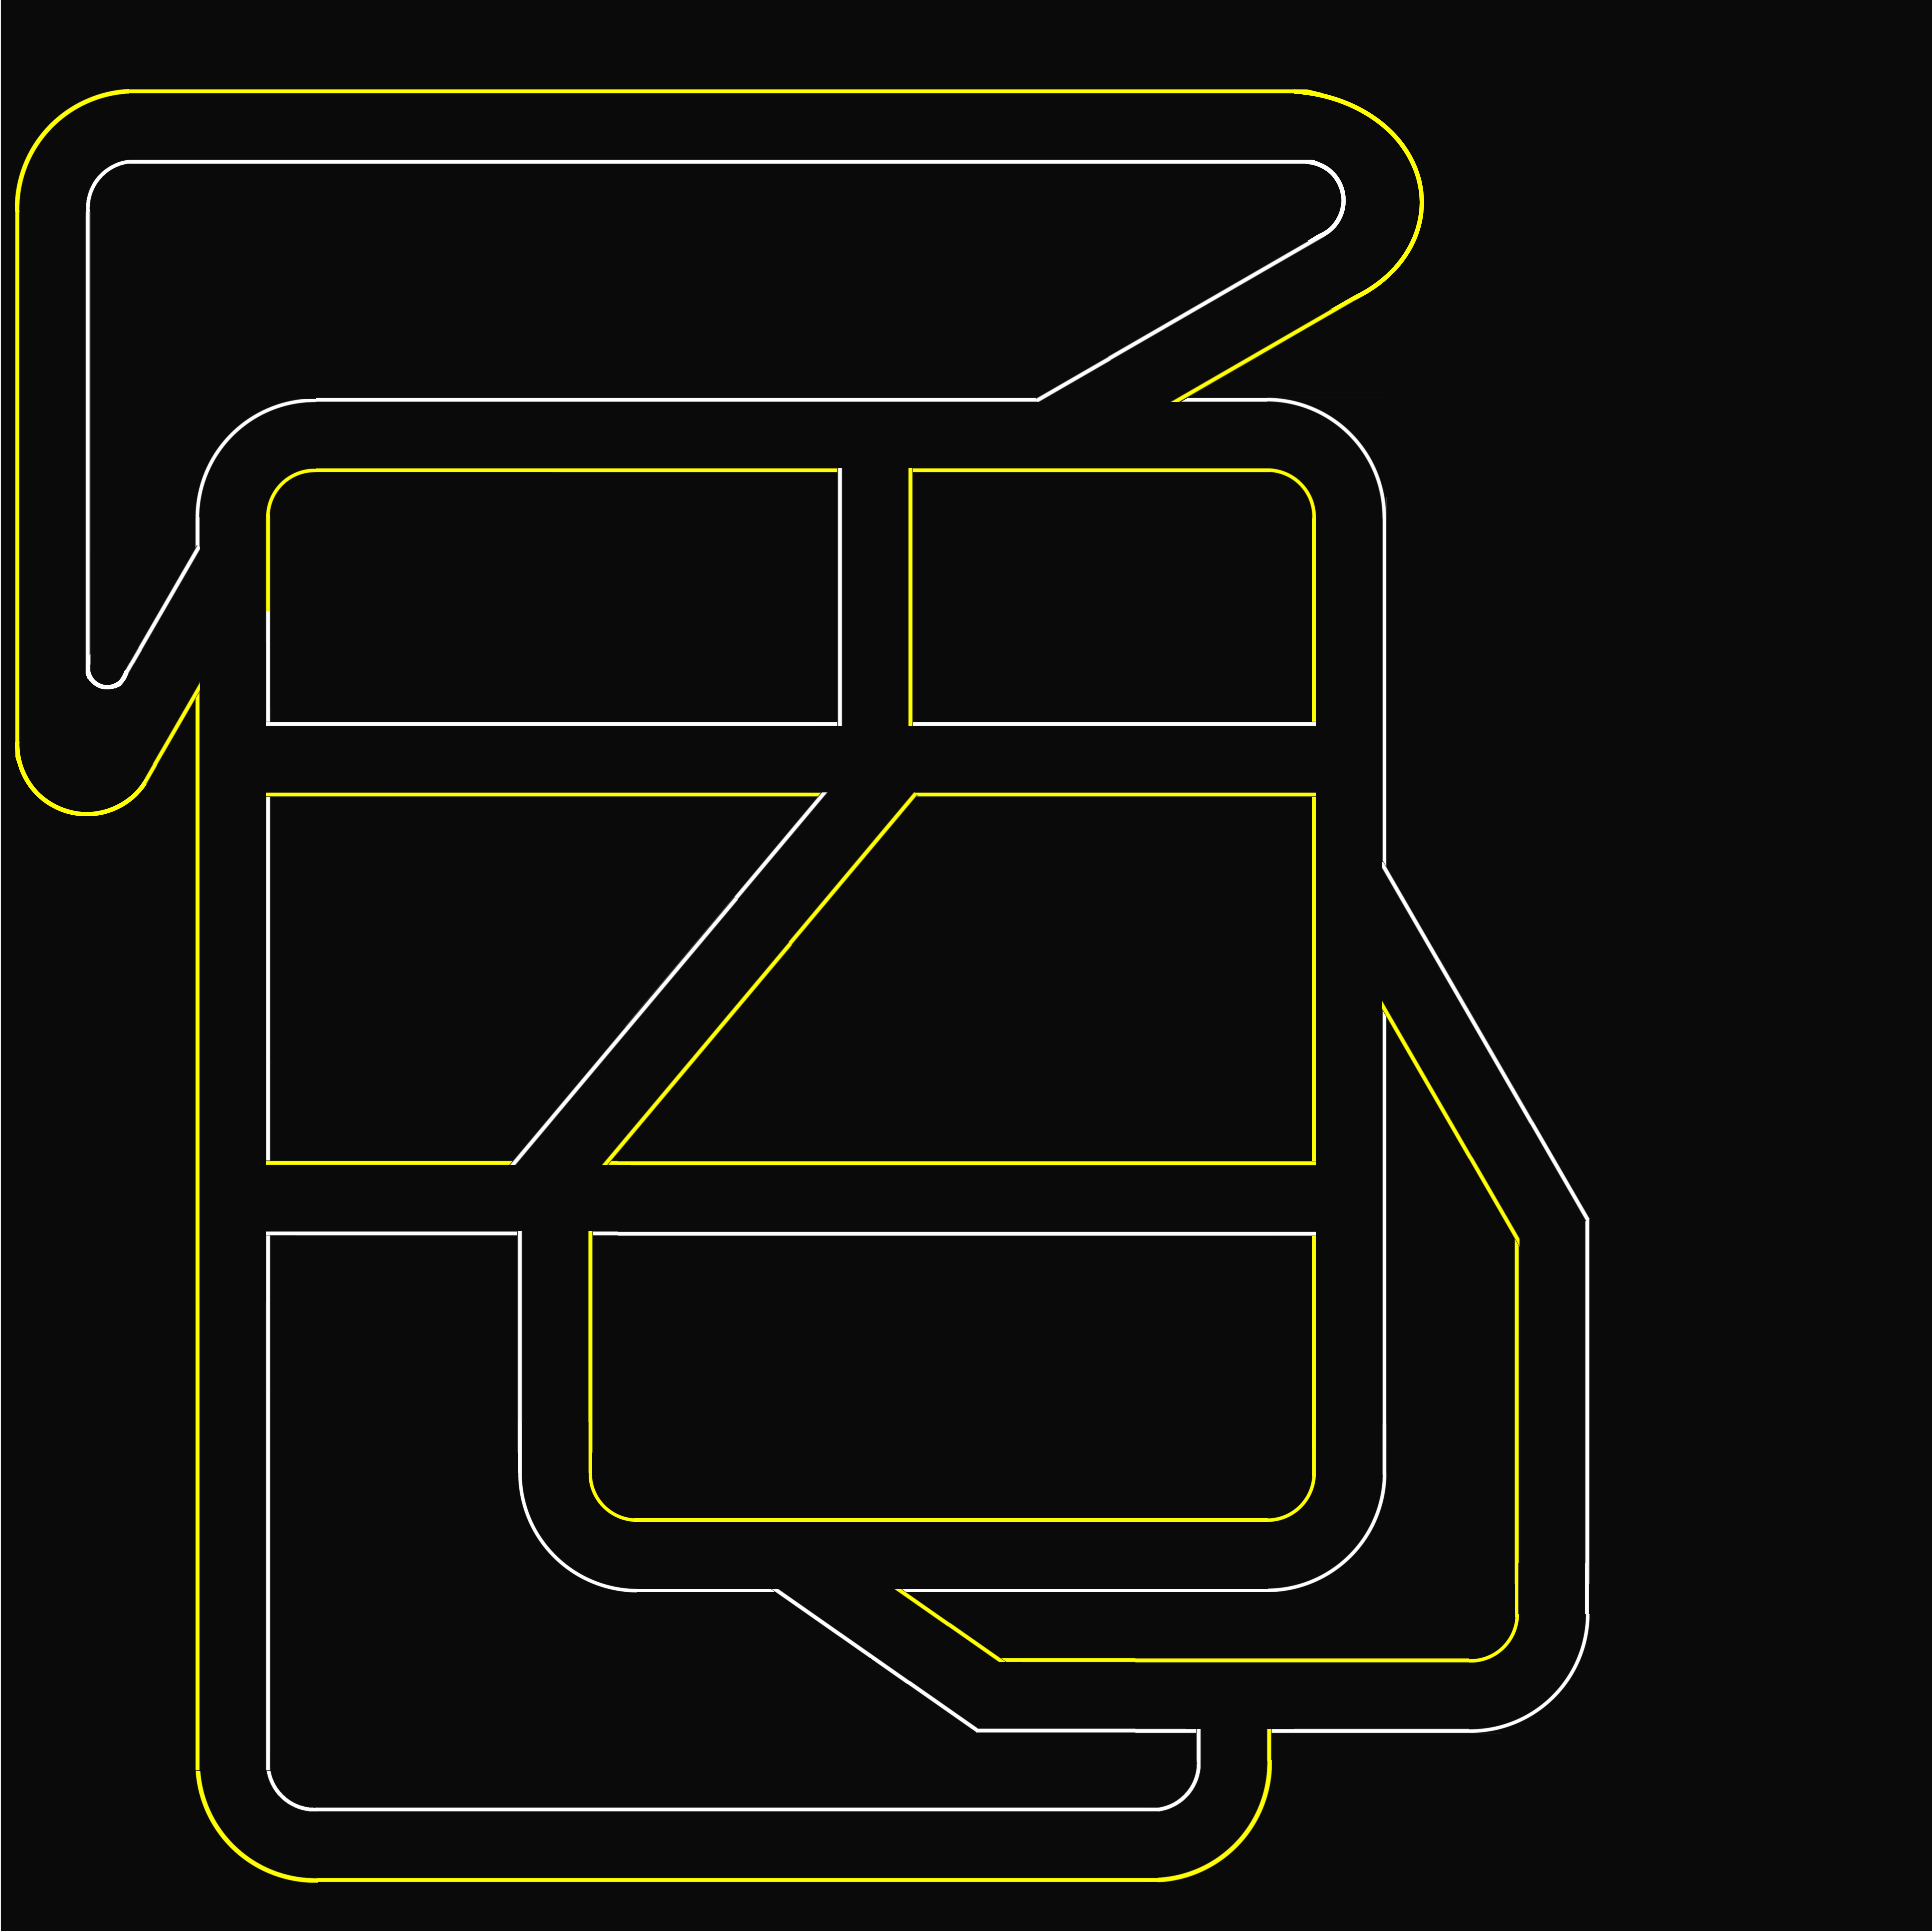
\includegraphics[height=0.5\textwidth]{images/road_final_map.png}
  \caption{Karte der finalen Testwelt mit Straßennetz}
  \label{fig:Testworld_Final_Map}
\end{figure}


\section{Anforderungen}
An dieser Stelle werden die Funktionalen Anforderungen (FA) beschrieben, welche die zu implementierenden Softwarekomponenten erfüllen müssen. Diese werden auf Basis des erläuterten
FunktionsMASTeRs beschrieben. In der Tabelle \ref{tab:requirements} werden alle Funktionalen Anforderungen erfasst, die das System mit der neuen Funktionalität umsetzen soll.
Die Anforderungen sind Grundlage für folgende Designentscheidungen und dienen als wesentliches Strukturelement für die Umsetzung.

Anforderungen die mit einem \textit{D} beginnen, haben die Hauptaufgabe etwas zu detektieren. Diese Anforderungen sollten von Detection-Nodes umgesetzt werden. Die Anforderungen, die mit
einem \textit{C} beginnen, sollen den Roboter kontrollieren. Entsprechend werden diese Anforderungen von Control-Nodes umgesetzt. 

Was in dieser Arbeit vernachlässigt wird, sind Nicht-Funktionale Anforderungen. Wie bereits erwähnt, beschreiben Nicht-Funktionale Anforderungen die Eigenschaften eines Systems.
Viele dieser Eigenschaften sind bereits identifiziert worden, wie z.B. die Programmiersprache oder Frameworks. Grundsätzlich handelt es sich bei diesem System um keines, welches produktiv
eingesetzt wird, wodurch eine Auseinandersetzung mit den Nicht-Funktionale Anforderungen des System nicht gerechtfertigt ist.


  \begin{table}
  
  \begin{adjustbox}{width=\textwidth}
  \begin{tabularx}{\textwidth}{@{} p{0.1\linewidth} p{0.8\linewidth} @{}}
    \textbf{ID} & \textbf{Anforderung} \\*
  \hline
    D1 & \textbf{Kreuzung erkennen} \\*
      & Selbsttätige Systemaktitivät \\*
      & Wenn sich der TurtleBot 3 einer Kreuzung nähert, muss das System diese erkennen. \\*
      & \textbf{Akzeptanzkriterien:} \\*
      & - das System stellt fest, dass es sich einer Kreuzung nähert und ändert den Modus \\
  \hline
    D2 & \textbf{Richtungen identifizieren} \\*
      & Selbsttätige Systemaktitivät \\*
      & Wenn das System eine Kreuzung erkannt hat, muss das System die möglichen Fahrtrichtungen bestimmen. \\*
      & \textbf{Akzeptanzkriterien:} \\*
      & - das System erkennt die Fahrtrichtungen und weiß, welche Fahrtrichtungen für eine Weiterfahrt erlaubt sind \\
  \hline
     D3 & \textbf{Schlüsselpunkte identifizieren} \\*
      & Selbsttätige Systemaktitivät \\*
      & Wenn das System eine Kreuzung erkannt und die Fahrtrichtungen identifiziert hat, muss das System die Schlüsselpunkte der Fahrtrichtungen bestimmen. \\*
      & \textbf{Akzeptanzkriterien:} \\*
      & - das System kann die Schlüsselpunkte einer Kreuzung berechnen \\
  \hline
     D4 & \textbf{Gegenverkehr identifizieren} \\*
      & Selbsttätige Systemaktitivät \\*
      & Das System muss in der Lage sein, Gegenverkehr zu identifizieren. \\*
      & \textbf{Akzeptanzkriterien:} \\*
      & - das System überprüft zu jeder Zeit, ob aktuell Gegenverkehr herrscht \\*    
      & - das System überprüft zu jeder Zeit, ob aktuell ein Fahrzeug im direkten Umfeld ist \\  
  \hline
    C1 & \textbf{Zur Kreuzung fahren} \\*
      & Selbsttätige Systemaktitivät \\*
      & Wenn das System die Schlüsselpunkte der Kreuzung berechnet hat, muss das System den Roboter zum Startpunkt der Kreuzung steuern. \\*
      & \textbf{Akzeptanzkriterien:} \\*
      & - der Roboter wird vom System mit einer minimalen Abweichung (unter 0.1 odom. Längeneinheit) zum Startpunkt gesteuert \\
  \hline
    C2 & \textbf{Abbiegen} \\*
      & Selbsttätige Systemaktitivät \\*
      & Wenn der Roboter vom System zum Starpunkt gesteuert wurde und kein Gegenverkehr existiert, muss das System den Roboter in eine erlaubte Richtung abbiegen lassen. \\*
      & \textbf{Akzeptanzkriterien:} \\*
      & - der Roboter kann mit einer minimalen Abweichung (unter 0.1 odom. Längeneinheit) zum Ausgangspunkt einer Kreuzung gesteuert werden \\
  \hline
  \end{tabularx}
  \end{adjustbox}
  \caption{Funktionale Anforderungen}
  \label{tab:requirements}
  \end{table}


\section{Softwarekomponenten}
Die zu implementierenden Softwarekomponenten sollen sich in das bestehende Projekt eingliedern. Dies vereinfacht die Lebenszyklen der zu implementierenden Nodes, da diese
nach ähnlichen Programmabläufen gestartet oder beendet werden, wie es für die bestehenden Nodes der Fall ist. Die Core-Nodes werden deshalb erweitert und neue Control- sowie
Detection-Nodes bereitgestellt.

\subsection{Control-Nodes}
Die Erweiterung der Core-Nodes beschränkt sich auf eine Erweiterung der Modi. Die Modi werden aktuell in einem Aufzählungstypen nachgehalten, \textit{CurrenMode}. Dieser Aufzählungstyp
wird durch den Wert \textit{control\_crossing} erweitert. Zusätzlich müssen die neuen Nodes abhängig vom Modus gestartet werden. Die neuen Nodes sollten in den Modi \textit{lane\_following}
und \textit{control\_crossing} in jedem Fall aktiv sein. 

\subsection{Detection-Nodes}
Insgesamt wird es zwei neue Detection-Nodes geben. Diese sind \textit{detect\_crossing} und \textit{detect\_traffic}. In Abbildung \ref{fig:DetectCrossing_Activity} ist das Aktivitätsdiagramm
der Node \textit{detect\_crossing} dargestellt. Grundsätzlich soll diese Node die Anforderungen D1, D2 und D3 umsetzen. Auslöser dieser Aktivität ist 
ein eingehenden Bild der Kamera des TurlteBot 3. Auf diesem Kamerabild wird zunächst die Aktion "Kanten detektieren"
durchgeführt. Ziel ist es, dass unwesentliche Bildelemente wie die Farbe oder Struktur der einzelnen Oberflächen aus dem Bild entfernt werden. Auf Basis des reduzierten Bildes können
im Folgenden Schritt die Geraden berechnet werden, die die einzelnen Kanten repräsentieren. Entsprechend der Voraussetzungen kann davon ausgegangen werden, dass eine Kreuzung
aus Geraden besteht, da ein Stück weit gerade Strecke vorhanden sein muss. Basierend auf dieser Prämisse, können aus den Kanten Geraden abgeleitet werden.
Diese Geraden werden nun geclustert. Damit die relevanten Intersektionen berechnet werden können, müssen die Geraden in einer Form gruppiert werden. Alle Geraden, die eine Fahrbahnbegrenzung
repräsentieren, sollten zusammen gruppiert werden. Im nächsten Schritt werden die Schnittpunkte und -winkel der Gruppen berechnet. Dies sind wichtige Informationen für den Roboter, 
um den Roboter gezielt abbiegen zu lassen. Weiterhin ist insbesondere der Schnittpunkt relevant, um die Schlüsselpunkte zu berechnen. Die Schlüsselpunkte sind hier für jede Richtung zu berechnen
und bestehen aus dem Start-Punkt sowie dem End-Punkt für das Abbiegemannöver. Diese Schlüsselpunkte sind zunächst aus den Bildkoordinaten abgeleitet und beschreiben somit einen Punkt
im konkreten Bild. Diese Koordinaten müssen im nächsten Schritt transformiert werden, sodass sie den odometrischen Koordinaten der Welt entsprechen. Nachdem alle Kerninformationen
berechnet wurden, muss bestimmt werden, welche Richtungen für eine Weiterfahrt erlaubt sind. Zusammenfassend werden die Daten noch gewichtet. Bei der Bildverarbeitung sind Abweichungen, auch
wenn sie minimal sind, einzukalkulieren. Wie bereits beschrieben kann dieses Problem bereits durch leichte Vibrationen entstehen. Ein zusätzliches Risiko sind falsch erkannte Daten.
Um einen guten Durchschnitt und falsche Erkenntnisse zu eliminieren, müssen ähnliche Resultate mit einer Wertung zusammengefasst werden. Diese Wertung beschreibt, wie wahrscheinlich 
es sich bei einem Resultat um eine Kreuzung handelt.
Im letzten Schritt werden die Resultate an das Topic \textit{detect/crossing/data} veröffentlicht.

\begin{figure}[h!]
  \centering
  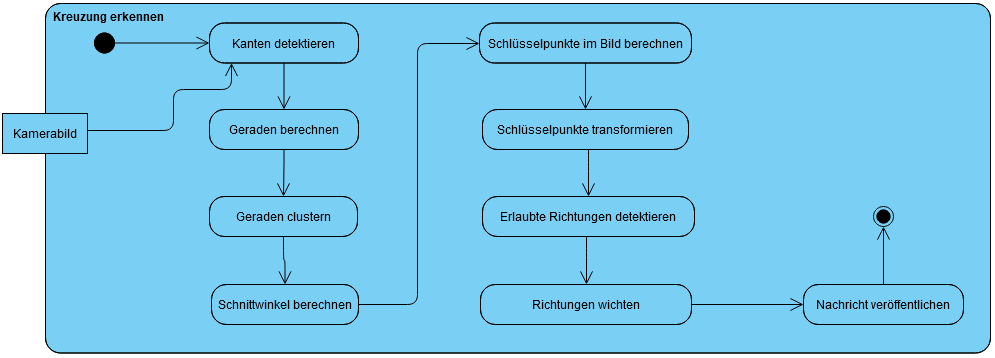
\includegraphics[width=\linewidth]{images/DetectCrossing_activity.PNG}
  \caption{Akitivitätsdiagramm der Node \textit{detect\_crossing}}
  \label{fig:DetectCrossing_Activity}
\end{figure}

Die zu versendende Nachricht wird durch eine Liste des in \ref{fig:msg-crossingdata} dargestellten ROS-Message-Formats repräsentiert. Diese Nachricht beinhaltet alle Informationen,
die durch den im Aktivitätsdiagramm beschriebenen Prozess berechnet wurden. Zusätzlich sind hier die Informationen \textit{angle\_to\_start} sowie \textit{angle\_at\_start} als Felder
der Nachricht deklariert. Diese Daten können ebenfalls aus den Schlüsselpunkten abgeleitet werden. Ziel hierbei ist zu wissen, in welche Richtung der Roboter fahren muss, damit 
der Startpunkt erreicht werden kann als auch wie der Roboter am Startpunkt ausgerichtet werden muss. 

\begin{code}
  \begin{minted}[
      baselinestretch=1.2,
      fontsize=\small,
      breaklines=true
  ]{python}
  string direction
  bool allowed
  float32 angle_to_start
  float32 angle_at_start
  float32 start_x
  float32 start_y
  float32 angle_target
  float32 angular_distance_target
  float32 target_x
  float32 target_y
  \end{minted}
  \quelle{eigene Darstellung}
  \caption{Message-Format für die Kreuzungsdetektion \textit{CrossingData}}
  \label{fig:msg-crossingdata}
\end{code}


Die Node \textit{detect\_traffic} wird zwei Aktivitäten zeitgleich ausführen und ist für die Anforderung D4 verantwortlich. Weiterhin ist zu bemerken, dass diese Node in jedem Modus
aktiviert sein sollte. Die erste Aktivität ist in Abbildung \ref{fig:DetectTraffic_Odom_activity} dargestellt.
Auslöser dieses Programmablaufs ist eine erhaltene Nachricht der vom Roboter veröffentlichten odometrischen Daten. Diese Daten sollen die Informationsgrundlage für Connected Cars
repräsentieren. Damit diese Daten für andere Roboter wiederverwendbar sind, ist es jedoch wichtig, dass diese Daten im Schritt "Daten taggen" gekennzeichnet werden. Als Kennzeichnung
wird wie bereits beschrieben eine UUID verwendet. Diese wird beim Start dieser Node generiert und ist für jede Instanz der Roboter eindeutig. Über diese ID sind die Bewegungen aller Roboter
für jeden einzelnen zuordenbar. Von der Idee ist diese Funktionalität in einer Detection-Node nicht richtig angesiedelt. Da jedoch hier auf Gegenverkehr und somit Kollisionen geprüft wird, ist
es leichter, wenn die Daten auch in dieser Node produziert werden. Zusätzlich existiert in der bestehenden Implementierung kein Node-Typ, in den diese Verantwortung passen würde.
Das Topic, an welches diese Daten veröffentlich werden, ist \textit{/detect/traffic/position}. Dieses Topic ist ein globales Topic. Das Nachrichtenformat ist in \ref{fig:msg-detecttrafficposition}
dargestellt und beinhaltet lediglich die odometrischen Daten sowie die ID des Roboters.

\begin{figure}[h!]
  \centering
  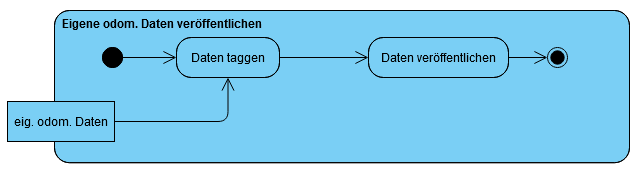
\includegraphics[width=\linewidth]{images/DetectTraffic_odom_activity.PNG}
  \caption{Akitivitätsdiagramm zum Taggen der Daten der Node \textit{detect\_traffic}}
  \label{fig:DetectTraffic_Odom_activity}
\end{figure}

\begin{code}
  \begin{minted}[
      baselinestretch=1.2,
      fontsize=\small,
      breaklines=true
  ]{python}
  string vehicle_id
  geometry_msgs/PoseWithCovariance pose
  geometry_msgs/TwistWithCovariance twist
  \end{minted}
  \quelle{eigene Darstellung}
  \caption{Message-Format für das Taggen der odom. Daten}
  \label{fig:msg-detecttrafficposition}
\end{code}

Die konkrete Analyse des Verkehrs ist in Abbildung \ref{fig:DetectTraffic_Danger_activity} zu sehen. Ausgangspunkt dieses Prozesses ist der Erhalt einer Nachricht mit getaggten odometrischen
Daten eines anderen TurtleBot 3. Zunächst werden anhand dieser Daten die Fahrbahnen berechnet. Hier wird angenommen, dass zu keinem Zeitpunkt eine angulare Beschleunigung von 0 existiert.
Falls doch, soll diese durch einen Wert, der sich 0 annähert, substituiert werden. Unter diese Annahme gilt, dass sich die Roboter zu jedem Zeitpunkt auf einer Kreisbahn bewegen.
Die einzelnen Fahrbahnen werden somit durch Kreise repräsentiert. Im zweiten Schritt werden die potenziellen Schnittpunkte dieser Kreise berechnet. Diese Schnittpunkte sind die Stellen,
an denen beide Roboter kollidieren würden. Anschließend wird auf Basis der Schnittpunkte und der aktuellen Position auf dem Kreis die Distanz zwischen dem Roboter und der Kollisionspunkte berechnet.
Falls hier eine Kollision möglich ist, soll eine Nachricht veröffentlicht und der Prozess beendet werden. Falls kein Schnittpunkt berechnet wurde, wird die Distanz zwischen dem aktuellen und
anderem Roboter berechnet, ähnlich zu einem Radar-System. Wenn sich das andere Fahrzeug innerhalb einer von der Welt abhängigen Distanz befindet, soll geprüft werden, ob die beiden Fahrzeuge
auf Basis ihrer aktuellen Ausrichtung aufeinander zusteuern. Wenn dies der Fall ist, wird ebenfalls eine Kollisions-Nachricht veröffentlicht und der Prozess beendet. Wenn sich die Roboter
nicht auf Kollisionskurs befinden, jedoch nahe beieinander sind, soll eine Warn-Nachricht veröffentlicht werden. Grundsätzlich sind hier ledigliche Fahrzeuge interessant, die sich vor
dem Roboter befinden. 

\begin{figure}[h!]
  \centering
  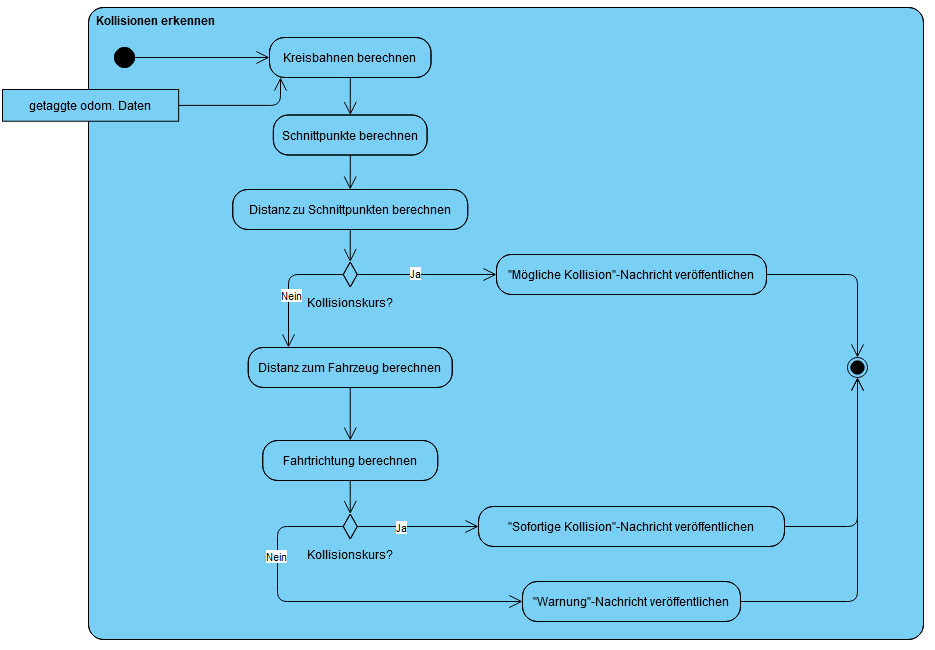
\includegraphics[width=\linewidth]{images/DetectTraffic_danger_activity.PNG}
  \caption{Akitivitätsdiagramm zur Kollisionserkennung der Node \textit{detect\_traffic}}
  \label{fig:DetectTraffic_Danger_activity}
\end{figure}

In \ref{fig:msg-detecttrafficcollision} wird das Nachrichtenformat für diesen Prozess definiert. Über das Feld \textit{collision\_type} wird identifizert, ob es sich um eine mögliche bzw.
sofortige Kollision oder aber nur um eine Warnung handelt. Zusätzlich werden in dieser Nachricht die odometrischen Daten des eigenen Fahrzeugs als auch des geprüften Fahrzeugs 
veröffentlicht. Im Falle, dass es zu einer Kollision kommt, wird in dem Feld \textit{time\_till\_collision} die Zeit und in \textit{distance\_till\_collision} die Distanz bis zur Kollision
übermittelt. Das Topic für diese Nachricht ist \textit{detect/traffic/collision}.

\begin{code}
  \begin{minted}[
      baselinestretch=1.2,
      fontsize=\small,
      breaklines=true
  ]{python}
  int32 collision_type
  geometry_msgs/PoseWithCovariance other_vehicle_pose
  geometry_msgs/TwistWithCovariance other_vehicle_twist
  geometry_msgs/PoseWithCovariance current_vehicle_pose
  geometry_msgs/TwistWithCovariance current_vehicle_twist
  int32 time_till_collision
  float32 distance_till_collision
  \end{minted}
  \quelle{eigene Darstellung}
  \caption{Message-Format für eine Kollision}
  \label{fig:msg-detecttrafficcollision}
\end{code}

\subsection{Control-Nodes}
Zusätzlich werden zwei Control-Nodes implementiert. Die erste Control-Node ist \textit{control\_traffic}, die zweite \textit{control\_crossing}. Ähnlich zu den Detection-Nodes
sollte auch hier die Node \textit{control\_traffic} unabhängig vom Modus generell aktiv sein. Die konkrete Aufgabe dieser Node ist es, auf potenziellen Gegenverkehr zu reagieren
und Kollisionen zu vermeiden. Zusätzlich hat diese Node die Verantwortung, Verkehrsregeln zu beachten und aufzulösen. Im Falle, dass sich zwei Roboter entsprechend \ref{Szenario 3} 
auf Kollisionkurs an einer Kreuzung befinden, soll diese Node die Situation durch die konkrete Verkehrsregel auflösen. In Abbildung \ref{fig:ControlTraffic_Activity} ist der Prozessablauf dieser Node abgebildet.
Auslöser dieses Prozesses ist eine Nachricht der Node \textit{detect\_traffic}. Auf Grundlage dieser Daten wird zunächst ermittelt, ob es sich überhaupt um eine zu behandelnde
Kollisionsnachricht handelt. Wenn dies der Fall ist, wird geschaut, wie dringend der Handlungsbedarf ist. Wenn die Roboter nah beieinander sind und aufeinander zusteuern, wird
die Aktivität "Drossel max. Geschwindigkeit" ausgeführt. Hierbei wird die maximale Geschwindigkeit auf 0 begrenzt, um den Roboter auf der Stelle anzuhalten. Diese Zustand wird beibehalten,
bis keine Kollisionsgefahr mehr besteht und die Weiterfahrt frei fortgesetzt werden kann. Ähnlich ist es, wenn eine Warnung besteht, weil sich beispielsweise ein anderer Roboter vor
dem gesteuerten Roboter befindet, der in die selbe Richtung fährt. Wenn der andere Roboter langsamer fährt, würde es auch hier zu einer Kollision kommen. Entsprechend eines Sicherheitsabstands
zwischen den Robotern sowie der Geschwindigkeit des anderen Roboters, soll eine neue Geschwindigkeit für den gesteuerten Roboter berechnet werden, sodass dieser nicht auffährt.
Sobald auch hier eine freie Weiterfahrt möglich ist, da der andere Roboter beispielsweise abgebogen ist, soll die Geschwindigkeitsbegrenzung des gesteuerten Roboters aufgehoben werden.

\begin{figure}[h!]
  \centering
  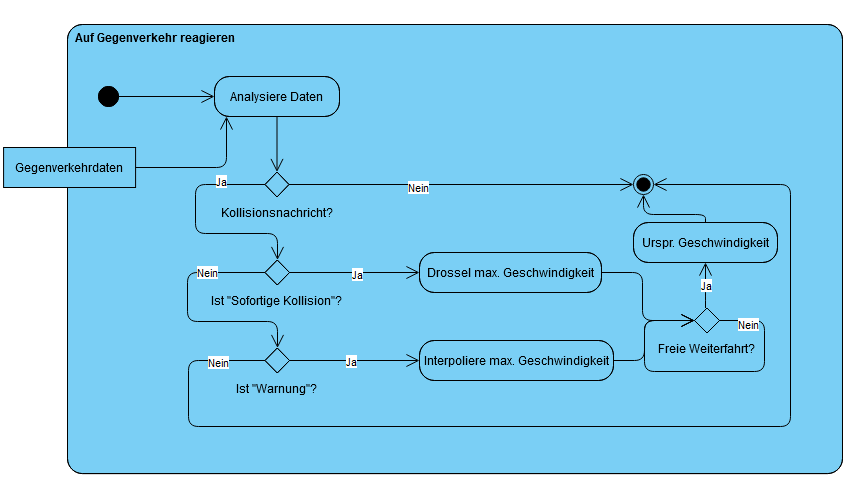
\includegraphics[width=\linewidth]{images/ControlTraffic_activity.PNG}
  \caption{Akitivitätsdiagramm zur Kollisionssteuerung der Node \textit{control\_traffic}}
  \label{fig:ControlTraffic_Activity}
\end{figure}

Der Prozess der Node Node \textit{control\_crossing} ist in \ref{fig:ControlCrossing_Activity} abgebildet. Auslöser dieses Prozesses sind Nachrichten aus der Node \textit{detect\_crossing}.
Die Hauptaufgabe dieser Node ist, den Roboter an einer Kreuzung zu steuern und den Roboter in eine Richtung abbiegen zu lassen. Dieser Prozess lässt sich in drei Schritte aufteilen.
Wenn eine Kreuzung mit ihren Schlüsselpunkten erkannt wurde, soll der Robter zunächst an den Startpunkt der Kreuzung fahren. Wenn der Roboter diesen Punkt erreich hat, wird er gestoppt und es wird
auf Gegenverkehr geprüft. Grundsätzlich hat die Node \textit{control\_traffic} diese Aufgabe. Wenn jedoch Gegenverkehr detektiert wurde und es sich dabei beispielsweise entsprechend \ref{Szenario 5}) 
um einen Roboter handelt, der eine Richtung durch stillliegen blockiert, sollte der Roboter eine alternative Route fahren. Sobald kein Gegenverkehr mehr vorhanden ist, kann der Roboter mit dem konkreten
Abbiegevorgang fortfahren. Hier soll der Roboter vom Startschlüsselpunkt zum Zielschlüsselpunkt fahren.


\begin{figure}[h!]
  \centering
  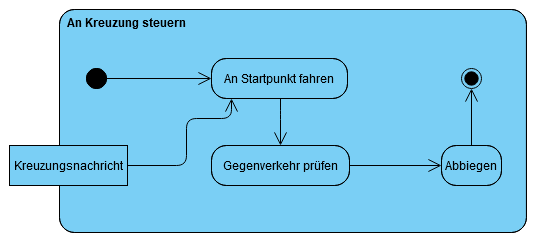
\includegraphics[width=\linewidth]{images/ControlCrossing_activity.PNG}
  \caption{Akitivitätsdiagramm der Node \textit{control\_crossing}}
  \label{fig:ControlCrossing_Activity}
\end{figure}